\chapter{Dictionaries}\label{chap:dict}

When you read Pāli text, an indispensable tool is dictionaries. So, a good Pāli text reader needs a good integration of good dictionaries. Unfortunately, we really have limited resources of Pāli dictionaries. All we have here, are all we can get in digital form. Most of them are rather old. A game changer recently is Digital Pāḷi Dictionary (DPD). This one is not bundled (see Chapter \ref{chap:dpd}).

The five dictionaries bundled with the program and ready to use are as follows:

\textbf{(1) Concise Pāli-English Dictionary (CPED).}\footnote{By Ven.\ A.\,P. Buddhadatta, available online at \url{www.budsas.org/ebud/dict-pe/index.htm}} This dictionary holds a significant position in the program. It is the only one that is structured and used widely in various contexts. I also made a few corrections and added some entries.

\textbf{(2) Concise English-Pāli Dictionary (CEPD).}\footnote{By Ven.\ A.\,P. Buddhadatta, available online at \url{www.budsas.org/ebud/dict-ep/index.htm}} This may be less used but has its own merit. It can give you a word that you do not know it in Pāli, but you know its close English terms. Although you can search in meanings of all dictionaries, simple searching in this dictionary is faster and sufficient in most cases.

\textbf{(3) New Concise Pāli-English Dictionary (NCPED).}\footnote{Compiled by SuttaCentral (\url{suttacentral.net}), updated and corrected from Margaret Cone's Dictionary of Pali} Since this dictionary is derived from CPED, so you can find redundancies here. But many entries are corrected and expanded. It is still concise and handy to use. Using this dictionary to recheck with CPED is a good idea. Unfortunately, Ven.\,Sujato told me that NCPED is now obsolete, no further update, and DPD is preferable to use instead.\footnote{Comparing the size and complexity of DPD and NCPED, I think NCPED still has its place in modern studies of Pāli. Sometimes, if not most of the time, I just need a simple search and just enough result, not mind-boggling details.}

\textbf{(4) The Pali Text Society's Pali-English Dictionary \\(PTSD).}\footnote{Originally this is written by T.\,W.\ Rhys\ Davids and W.\ Stede (1921--25). It is subsequently revised in accordance with the 2015 ``Reprint with corrections'' by K.R.\ Norman, William\ Pruitt and Peter\ Jackson. The digital version is released by \emph{Buddhadust} (\url{buddhadust.net}), proofread 2021. For more information, see \url{vpnry.github.io/ptsped}.} This a little outdated dictionary is still indispensable and often gives some insight to the words we study.

\textbf{(5) Dictionary of Pāli Proper Names (DPPN).}\footnote{By Gunapala Piyasena Malalasekera, available online at \url{www.palikanon.com/english/pali\_names/dic\_idx.html}} You may seldom use this one. It gives detailed information about Pāli names, not directly the explanation of the terms.

\bigskip
Apart from the five above, you can see another dictionary named MDPD (Mini-DPD). This one will be newly created when you get DPD and process it for the first time. This dictionary is much more concise than the full DPD and can be used with search functionality along with other dictionaries.

\section{Using dictionaries}

Before you can use a dictionary mentioned above, you have to create its data first. This is because the program is only shipped with raw dict data in CSV format. These data have to be converted into tables in Dict database. Normally, creating dict data is a very first action you do when you successfully make the program run for a serious use. To do this is simple, just select menu Dict > {\faSix \symbol{"F1C0}} Create Dict data, and wait for a while until the Dict engine is ready.

\dothis{Before you can use any of dictionaries bundled with the program, select this in the menu:\\
\menucommand{Dict > {\faSix \symbol{"F1C0}} Create Dict data}
\begin{center}\rule{0.5\linewidth}{1pt}\end{center}
After the dict data are created, it is a good practice to lock the Dict database by toggling this menu:\\
\menucommand{Dict > {\faSix \symbol{"F09C}} Dict DB unlocked}\\
to\\
\menucommand{Dict > {\faSix \symbol{"F023}} Dict DB locked}\\
\\
Now then the menu of {\faSix \symbol{"F1C0}} Create Dict data will be disabled.
}

After Dict data are available, now you can open a Dict window (or use the Dict tab) and enter a search query. To open a Dict window, see the instruction box below.

\dothis{To open a Dict window, press {\faSix \symbol{"F02D}} button in the main tool bar, or select this menu:\\
\menucommand{Dict > {\faSix \symbol{"F02D}} Dictionaries}
}

Once you enter a query in the search field, the search is done immediately. This can take time for the first letter because a lot of terms have to be retrieved. When a subsequent letter is entered, the result will be narrowed down quickly. An example of this can be seen in Figure \ref{fig:dictionaries}. This incremental search is the default mode. If you feel inconvenient, you can use the wildcard mode (see below).

\begin{figure}[!hbt]
\centering
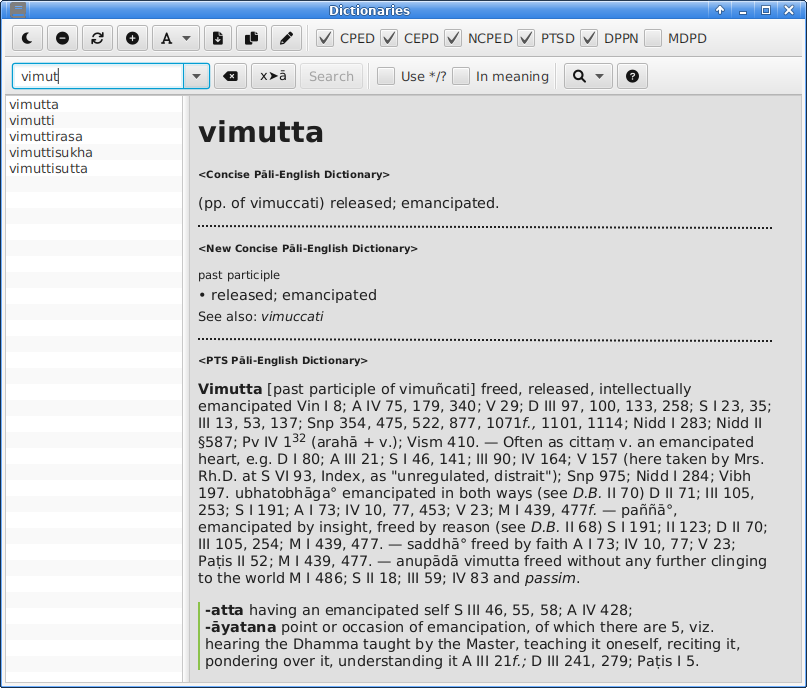
\includegraphics[width=0.9\linewidth]{images/dictionaries.png}\\
\caption{Dictionaries window and its result}
\label{fig:dictionaries}
\end{figure}

On the top of Dict window, you can see check boxes used for including dictionaries in a search. The selection is temporary. For persistent setting, consider using Settings window as shown in Figure \ref{fig:settings-dict}.

\begin{figure}[!hbt]
\centering
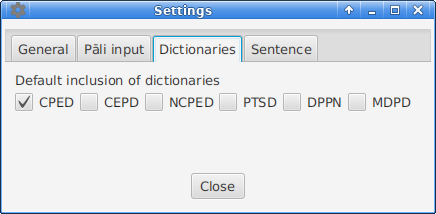
\includegraphics[width=0.6\linewidth]{images/settings-dict.png}\\
\caption{Default dictionary selection}
\label{fig:settings-dict}
\end{figure}

\section{Dictionary search modes}

Searching in Dictionaries can be one of the following four use cases:

\subsection*{1. Simple search}

Simple search is fast and simple. You enter some characters, the relevant results will be listed immediately, and the topmost entry is shown in the result area. Figure \ref{fig:dictionaries} shows the result of a simple search. Technically, this is called incremental search, and it takes time for the retrieval of the first letter.

\subsection*{2. Wildcard search}

Sometimes you have a vague idea what the word looks like. You can use wildcard mode by enabling \textbf{Use */?}. In this mode you can use ? to stand for any one character and * to stand for any characters (including none). Figure \ref{fig:dictionaries-wildcards} shows the result of searching `*mutt?'. Remember that in wildcard mode the result does not come up immediately. You have to press Search button or hit the Enter key.

\begin{figure}[!hbt]
\centering
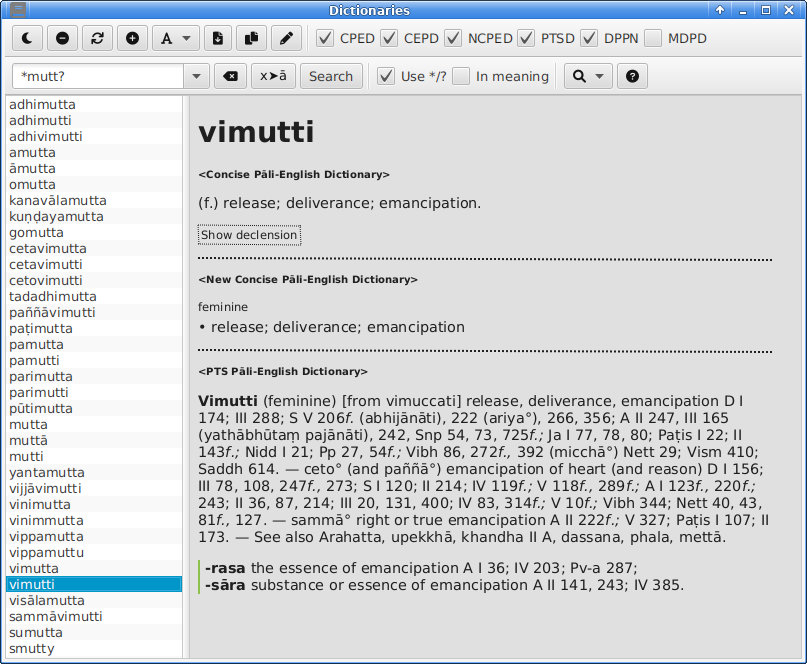
\includegraphics[width=0.9\linewidth]{images/dictionaries-wildcards.png}\\
\caption{Wildcard search in Dictionaries}
\label{fig:dictionaries-wildcards}
\end{figure}

As shown in the picture, * can mean zero character, and ? always represents one character. So, we also see \pali{mutta, muttā,} and \pali{mutti} in the result list. In the result of CPED, if the selected term is declinable (either noun or adj.), we will see \fbox{Show declension}. When we click this box-button, a declension window of that term will be opened.

\subsection*{3. Meaning search}

Yet sometimes you have no clue what the word should be. In this case, searching in the meanings of dictionaries can help. Figure \ref{fig:dictionaries-meaning} shows the result of searching `emancipate.' In this mode, using wildcards is not allowed, and do not forget to press Search button or hit Enter to submit the query.

\begin{figure}[!hbt]
\centering
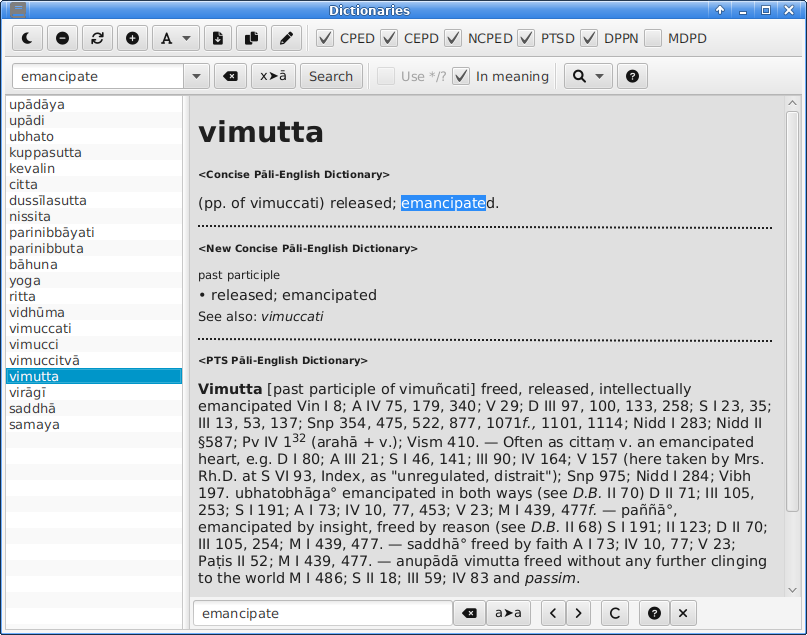
\includegraphics[width=0.9\linewidth]{images/dictionaries-meaning.png}\\
\caption{Dictionaries' meaning search}
\label{fig:dictionaries-meaning}
\end{figure}

Because of a technical limitation in highlighting the search result when you search in meanings, you have to find the word you are looking for by yourselves using \texttt{Ctrl-F} (see the result in Figure \ref{fig:dictionaries-meaning}). See more instruction in the box below.

\dothis{To find a string in search result, press \texttt{Ctrl-F} or select from this menu button in the Dict tool bar:\\
\menucommand{{\faSix \symbol{"F002}} > Find}\\[2mm]
\hspace{5mm}Or you can open the whole result in a program's Editor by pressing {\faSix \symbol{"F303}} button on the top tool bar.
}
